%!TEX root = ../thesis.tex

\chapter{Method}

\section{Implementation}
A common application where GPGPU is used is when computing calculation heavy simulations such the N-Body problem described in this thesis. Other common visualizations where GPGPU can be applied is to visualize fractals such as the Julia or Mandelbrot set, named after the french mathematician Gaston Julia and Benoit Mandelbrot. GPGPU has also been used in medicine for accelerated medical image reconstruction \cite{archirapatkave2011gpgpu}, as well as accelerating the Marching Cubes algorithm \cite{johansson2006accelerating}. 

This section describes the implementation of the visualization and the parallel N-Body algorithm in all discussed frameworks, as well as how the measurements were performed and what framework specific features was used. All implementations was implemented in C/C++. The visualization was implemented in the cross-platform API OpenGL on a Windows PC.

\section{Visualization} \label{sec:visualization}

Although not necessary for the evaluation, a visualization of the system was implemented. This was the first step in the implementation process, and the visualization was made using OpenGL. The purpose of the visualization is to make it easier to test and debug the application, which is very difficult without a proper way of visualizing the calculated positions. The N-Body visualization is very similar to a particle system, where each body is represented by a particle. To be able to visualize a very large amount of bodies, the visualization performance is critical, and there are a few ways of implementing a particle system in OpenGL.

The first, and perhaps the most intuitive way is to render a sphere in all positions, by calling \lstinline{glDrawArrays} N times e.g. in a for-loop. This is very inefficient in two regards; a sphere requires a lot of vertices to appear smooth, and drawing a large amount of spheres requires a large amount of vertex data. The second reason this is inefficient is because all SM's (Streaming Multiprocessor) on the GPU will be dedicated to drawing a single polygon, resulting in a huge amount of performance loss. However, since the particles are so small, they don't have to be rendered with a high resolution. A commonly used trick when rendering particle systems is to represent each particle as a quad with a semi-transparent texture with a circle. Each particle will thus only consist of four vertices, which is far less than if each particle was represented by a sphere. The quad is then rotated so that the quad's always faces the camera, giving the illusion that the particle is actually a sphere (or whatever shape the texture represents). This technique is known as \textit{billboarding}.

\nomenclature[z-SM]{SM}{Streaming Multiprocessor}

The solution to the second problem is a bit more complex, and a few solutions exists.
One way is to generate a single vertex buffer object (VBO) with all the particles in them. This is a easy and effective solution that works on all platforms. 

The second way is to use geometry shaders to render a particle in each position. The downside to using geometry shader is that geometry shaders is only supported in systems with OpenGL version 3.2+, and is thus not very portable. 

The third way is to use instancing, meaning that a single mesh is used, but many instances of the mesh. This solution has a nice balance between performance and availability and was thus chosen in this implementation. To achieve this, two main VBO's are used: one VBO containing the positions of the quad, i.e. four vertex coordinates, and a second VBO of size $n$ containing the positions of the instances of the quad, where $n$ is the number of instances. The quad is then rendered using \lstinline{glDrawArraysInstanced(GL_TRIANGLE_STRIP, 0, 4, n)} \cite{OpenCLDocs}, where the first parameter states that the object should be rendered as a triangle strip, i.e. a series of connected triangles, sharing vertices. The second parameter specifies the starting index in the enabled arrays. The third parameter specifies the number of indices to be rendered, and the fourth the number of instances. The quad positions are passed to the vertex shader as an attribute, and the shader then translates the quad into its position. The result of the implementation can be seen in figure \ref{fig:OpenGLEarlyVis}, where $n=3.5 \times 10^6$, running at a stable ~60fps on a Nvidia GTX970 GPU. Each quad is rendered in a random $(x,y,z)$ position in a given bounding box.


\begin{figure}[!htpb]
    \centering
    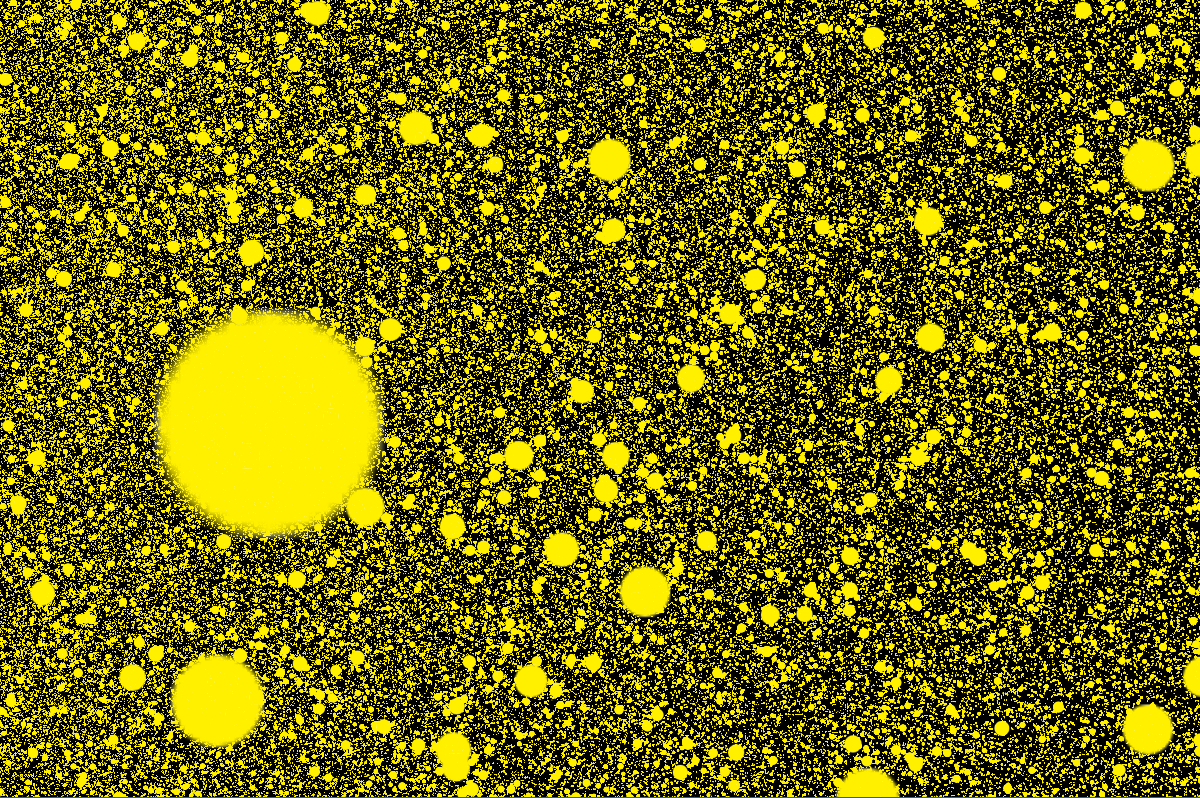
\includegraphics[width=0.8\textwidth]{Method/Figs/OpenGLVis_N=3500000.png}
    \caption{Instanced quad rendering, N=3.5*10^6}
    \label{fig:OpenGLEarlyVis}
\end{figure}


\section{Sequential}

This section will describe how a sequential implementation of the all-pairs N-body algorithm was implemented, followed by an optimized sequential implementation using the Barnes-Hut method. \cite{barnes1986hierarchical}


\subsection{All pairs implementation}
With the particle system visualization implementation described in section \ref{sec:visualization} as a template, a sequential all-pairs N-Body simulation was implemented. A particle is represented by a data structure which contains the position, velocity and mass of the particle. These particles are then instantiated and given a random position. All particles are given the same amount of mass, which makes it easier to analyze the simulation. To make the visualization more visually interesting, the particles are placed in a galaxy like structure using polar coordinates using a random $\varphi$ angle, and a random radius $r$ such that $x = r \ cos \ \varphi, \ y = r \ sin \ \varphi$. If the particles index is even it is translated with a constant length in the positive x-direction, whilst if the index is odd, it is translated in the negative x-direction resulting in two separated galaxy shapes.

To further mimic the behavior of a galaxy, each particle is given a speed according to:
\begin{equation}
    \boldsymbol v = (\boldsymbol c - \boldsymbol p) \times  \boldsymbol z
\end{equation}
\noindent where $\boldsymbol v$ is the velocity of the particle, $\boldsymbol c$ is the center of the galaxy, $\boldsymbol p$ is the position of the particle and $\boldsymbol z$ is the $z$ vector $(0, 0, 1)$. This results in that each particle will spin around the center of the galaxy, simulating how stars in a real galaxy behaves.

Once the system has been initialized, the integration is done in two separate steps. First, calculate the net force $F$ on each particle, as it is affected by gravity from all others according to equation \ref{eq:totGravForce}. In a sequential all-pairs implementation, this is done by using a nested for-loop resulting in a time complexity of $O(n^2)$. The next step is to update the position of the particle which is done using a first order Euler integration according to:
\begin{equation} \label{eq:EulerIntegrationPosition}
    \boldsymbol p' = \boldsymbol p + F * \Delta t
\end{equation}
\noindent where $p'$ is the new particle position, $p$ is the old position, $F$ is the net force applied to the particle and $\Delta t$ is the delta time of the simulation.
Since this is a first-order method, the error grows quickly with a local error proportional to the square of the step size, and a global error proportional to the step size. The step size of the Euler method used in this simulation does thus depend on the delta time which may vary on different systems. To prevent this a constant $\Delta t = c$ is used, with a small enough constant $c$ so that the integration is accurate enough. This simulation does not aim to be an physical accurate simulation so this integration method works well in this implementation.


\subsection{Octree construction} \label{subsec:OctreeConstruction}
The next step in the implementation was to start working on the Barnes-Hut algorithm by creating an octree from the particles in the particle system. This procedure follows the theory described in section \ref{subsec:BarnesHut} and illustrated in figure \ref{fig:BarnesHutTree}. The octree is represented as a data structure containing the spatial bounds of the cell, the spatial position of the node's center of mass, as well as the total mass contained in the node. It also contains it's eight children, which are of the same kind of data structure, thus resulting in a recursive data structure. The first step to building the tree is to find the bounds of the entire particle system, which is done in a simple reduction algorithm. With this information, the root node of the octree can then be constructed with the given bounds. The next step is to insert the positions of the particles which is done recursively. The position of the particle to be inserted is passed as an parameter, and the tree is then recursively traversed to find the respective node to insert the particle in. If this node is found to be already occupied with another particle, the node is then subdivided into eight new nodes, and the two particles are then moved into their respective new node. 

A problem with the insertion is to know what octant the particle should be inserted to. Since there are eight octant's this can be represented as a single byte. By comparing the position to be inserted with the middle of the cells x,y,z dimensions, this problem is reduced to a single binary expression by following a set of fixed rules. Pseudocode for this procedure can be seen in algorithm \ref{alg:OctreeBuild}, the procedure \lstinline{insert} is called for the root of the tree once for each particle. The resulting octree applied to a system with 2048 particles is visualized in figure \ref{fig:OctreeVisualized}.

Once the tree has been constructed, the next step is to calculate each nodes center of mass (COM) and the total mass contained inside the spatial domain that the node represents. This is again done by utilizing recursion. Each nodes COM is the average of it's children's COM and its total mass is the sum of it's children's total mass. The algorithm starts by calculating the root's COM and total mass, which recursively steps through the tree, calculating the COM of each nodes as it traverses the tree. The termination condition of the recursiveness is when a leaf node, or a uninitialized empty cell is reached.

\nomenclature[z-COM]{COM}{Center of Mass}

\begin{figure}[!h]
    \centering
    \begin{subfigure}[b]{0.65\textwidth}
        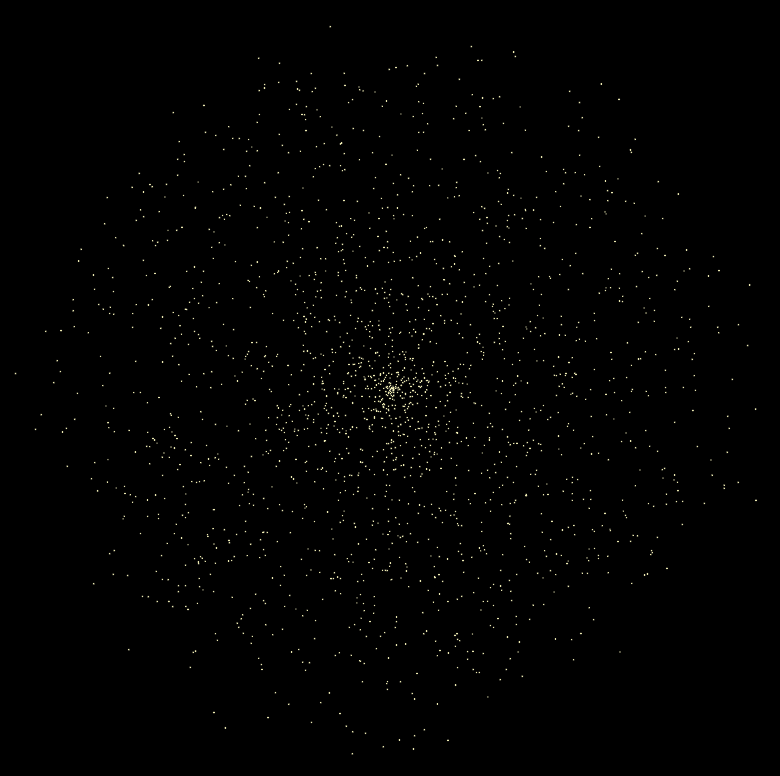
\includegraphics[width=\textwidth]{Method/Figs/PSNoBounds.png}
        \caption{Particle system}
    \end{subfigure}
    ~ 
    \begin{subfigure}[b]{0.65\textwidth}
        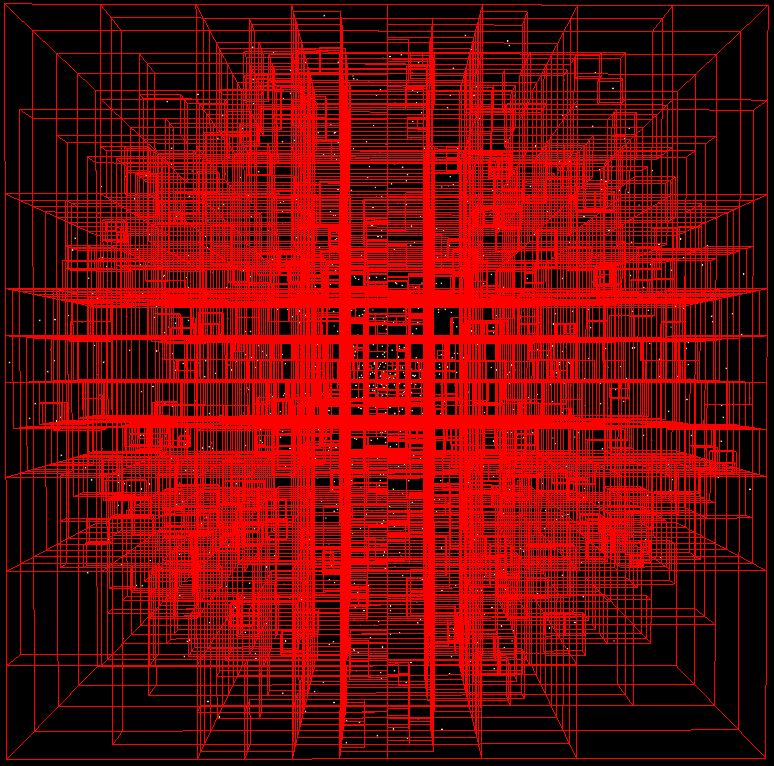
\includegraphics[width=\textwidth]{Method/Figs/PSWithBounds.png}
        \caption{Above particle system with rendered octree bounds}
    \end{subfigure}
    \caption{Particle system subdivided into an octree}
    \label{fig:OctreeVisualized}
\end{figure}


\begin{algorithm}[!h]
    \caption{Building octree pseudocode}
    \label{alg:OctreeBuild}
    \begin{algorithmic}[1]
    
    \Procedure{Insert}{$x, y, z, data$}
        \If{$node.isEmpty$}
            \Comment{Turn into leaf}
            \State $node.posx := x$
            \State $node.posy := y$
            \State $node.posz := z$
            \State $node.data := data$
        \Else
            \Comment{Node already contains data}
            \If{$node.isChild$}
                \Comment{Subdivide and move into appropriate child}
                \State \Call{InsertSub}{$node.posx, node.posy, node.posz, node.data$}
                \State $node.data = NULL$
            \EndIf
            \State \Call{InsertSub}{x,y,z, data}
        \EndIf
    \EndProcedure
    
    \Procedure{InsertSub}{$x,y,z, data$}
        \State $sub := 0$
        
        \If{$x > midX$}
            \Comment{Children 0,2,4,8 have positive x-coordinates}
            \State $sub += 1$
            \State $newMinX := midX$
            \State $newMaxX := maxX$
        \Else
	        \State $newMinX = minX$
		    \State $newMaxX = midX$
        \EndIf
        
        \If{$y > mid_y$}
            \Comment{Children 0,1,3,4 have positive y-coordinates}
    		\State $sub += 2$
    		\State $newMinY := midY$
    		\State $newMaxY := maxY$
    	\Else
    		\State $newMinY := minY;$
    		\State $newMaxY := midY;$
    	\EndIf
    
    	\If{$z > midZ$}
    	    \Comment{Children 0,1,2,3 have positive z-coordinates}
    		\State $sub += 4$
    		\State $newMinZ := midZ$
    		\State $n_max_z := maxZ$
    	\Else
    		\State $newMinZ := minZ$
    		\State $newMaxZ := midZ$
    	\EndIf
    	
    	
    	\If{!children[sub]}
    	    \Comment{$sub$ will now contain the octant index,  $sub \in {0,8}$}
        	\State \begin{varwidth}[t]{\linewidth}
                $children[sub] := new OctreeNode($ \par
                \hskip\algorithmicindent $newMinX, newMinY, newMinZ,$\par
                \hskip\algorithmicindent $newMaxX, newMaxY, newMaxZ)$
            \end{varwidth}
            
        \EndIf
	    \Call {$children[sub]->insert$}{$x, y, z, usr_data$}
        
    \EndProcedure
        
    \end{algorithmic}
\end{algorithm}    


\subsection{Barnes-Hut force calculation}
Once the tree has been built and the COM of each node has been calculated, the force calculation can begin. Besides the tree, an container containing information about all particles in the systems is used to simplify the data management. Each particle in this container is similar to that of the cells in the tree described in section \ref{subsec:OctreeConstruction}. The particle data structure contains information about the particles mass, position and velocity. This makes the force calculation simpler since the tree can be traversed once for each particle when calculating its net-force, which is a procedure that can easily be parallelized. 

The force calculation for a particle $p$ starts by traversing the tree from the root and then recursively traverses the tree. For each node it traverses, the euclidean distance from the particles position to the COM of the current node is calculated according to: 

\begin{equation} \label{eq:EucDist}
    d(\boldsymbol q, \boldsymbol p) = d(\boldsymbol p, \boldsymbol q) = \sqrt{(p_x-q_z)^2 +(p_y - q_y)^2 + (p_z - q_z)^2}
\end{equation}

\noindent where $q$ and $p$ is the position of the particle and the node. If this distance is equal to zero, it means that the current node is the same node as the particle, and the traversal continues. If the COM of the node is far away enough, the entire sub-tree of the node can be approximated as a single point mass and the force can be calculated using the COM and the mass of the node. If the node is to close to the particle, the sub-tree has to be "opened" and the traversal continues through the sub-tree, recursively calculating the net-force as the tree is traversed. 

One of the problems with the force calculation is what the distance that decides if a node is far away enough so that the sub-tree can be approximated should be. Barnes. et. al. does not mention a general strategy how this distance condition is specified  \cite{barnes1986hierarchical} . Burtscher et. al. uses a constant cutoff distance, which specifies when a node is far away enough \cite{burtscher2011efficient}.
This implementation uses a more general approach to this problem. The average width of the nodes bounds is calculated according to equation \ref{eq:Wavg}, where the max and min variables represent the bounds of the current node. The calculated average width is then used to calculate the ratio between the width and the distance to the node. If this width-to-distance ratio is smaller than a constant $c$, the node is considered to be far away enough to be evaluated as a single point. 

\begin{equation} \label{eq:Wavg}
    \begin{split}
    W_{avg} = &((max_x - min_x) + \\
              &(max_y - min_y) + \\
              &(max_z - min_z)) / 3 \\
    \end{split}
\end{equation}

When the net-force for all particles have been calculated, the position of the node is updated. It is important that this step is done after all of the forces have been calculated to get a correct simulation.
When the forces are calculated, the velocity property of each particle is updated. The position update is then simply done by applying equation \ref{eq:EulerIntegrationPosition} for each particle. With the position update, the simulation step is concluded. The tree is deallocated before beeing rebuilt the next simulation step. 

\section{CUDA} \label{sec:CUDAImplementation}
Once a sequential implementation was in place the work on porting the implementation to CUDA was started.
The octree data structure was built using pointers, pointing to its child sub-trees. This creates two problems when copying the tree structure to the GPU. The first problem is that the size of the tree is unknown and changes very frequently as the tree is rebuilt every simulation step, resulting in an uncertain amount of data to be transferred to the device. Although the size of the tree can be calculated, either when the tree is beeing built, or by a simple depth- or breadth-first traversal of the tree once the tree has been constructed. This solution does however only solve the first problem.

The second problem is that pointers in the octree point to a memory location in the heap memory, which when transferred to the device must be updated to point at the correct position in the VRAM memory, which would be a performance heavy task. Moreover, complicated structures involving a lot amount of pointers works poorly performance-wise in CUDA, since all the pointer chasing might drastically decrease the total memory bandwidth. 

The solution to both problems is to flatten the tree into an array with a fixed size $n > N$, where $N$ is the number of bodies. The tree will have $N$ leaves, so the size of the array has to have a fixed size which is bigger than the amount of bodies. Implementation wise this was done in two steps.
The first step was to do an iterative breadth-first traversal of the tree, starting from the root, and inserting the traversed nodes into the array, as well as assigning the index to each node. This results in that the array will be sorted top-down, left-right from the tree with the root at index one, visualized on a binary tree in figure \ref{fig:BreadthFirstTreeIndices}. Now that the tree has been flattened into a single list, the child pointers of each node can be replaced with the indices of the child nodes which lies in the same list as the node, making the requirement of pointers in the CUDA kernel redundant and avoiding the the pointer chasing issue.

\begin{figure}[!h]
    \centering
    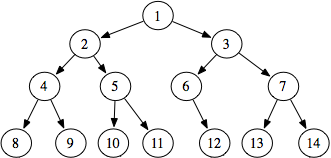
\includegraphics[width=0.6\textwidth]{Method/Figs/breadthFirstTree.png}
    \caption{Order of the flattened tree when a breadth-first flattening algorithm is applied to a binary tree}
    \label{fig:BreadthFirstTreeIndices}
\end{figure}


Now that the octree has been flattened into a tree, it can effortlessly be copied to the device since both the size of the flattened tree is known, and the pointers to each nodes children has been abstracted away and been replaced with indices in the flattened tree, and since CUDA supports the ability of passing class objects to a kernel, the flattened array consisting of octree nodes could simply be passed to the kernel as an argument. 

The remaining part of the algorithm is now reduced to two well parallelizable problems. The first is to calculate the net force of each particle, and the second to update the positions of each particle. The sequential force calculation handles one particle at a time, and traverses the tree once for each particle. This problem is well parallelizable by letting each thread handle one particle. The position update was parallelized in a similar fashion, each thread updates the position of a particle in parallel by using the Euler integration method described in equation \ref{eq:EulerIntegrationPosition}.

The sequential algorithm which was implemented before the CUDA implementation started utilizes recursion to traverse the tree when calculating forces. All Nvidia GPU's of compute capability 2.0 and higher support a stack and can thus utilize recursive functions in CUDA, making the tree traversal in the kernel very similar to the sequential tree traversal. However since recursive calls can't be inlined, and since the amount of overhead spawned when allocating memory for the recursive calls increases, they might significantly decrease the performance due to the spawned overhead when using recursion. Thus an iterative tree-traversal was implemented as well in a breadth-first fashion. The standard and most popular way of doing an iterative breadth-first traversal is by using a queue. All children of the active node is pushed onto the queue, and each iteration the first element in the queue is selected, iteratively pushing each nodes children onto the queue. CUDA does not support the use of the \lstinline{std::queue} in kernel code, so a manual FIFO (First In, First Out) queue data-structure was implemented which was used to implement an iterative tree traversal CUDA kernel.
Since CUDA supports C++ in kernels the queue could be implemented as a datastructure, containing expected member functions such as \lstinline{push(), pop()} etc. To avoid pointer chasing, the queue is implemented using an array as well as integers indexing the front and the back of the queue. The code for the queue can be seen in listing \ref{lst:MyQueue}.




\clearpage
\begin{lstlisting}[caption={Device queue used for iterative traversal of the tree}, label={lst:MyQueue}, frame=single] 

struct MyQueue {
	static const int MAX_SIZE = 10000;
	int f = -1, r = -1;
	int A[MAX_SIZE];

	bool empty() {
		return (f == -1 && r == -1);
	}
	bool isFull() {
		return (r + 1) % MAX_SIZE == f ? true : false;
	}
	void push(int x) {
		if (isFull()) {
			return;
		}
		if (empty()){
			f = r = 0;
		}
		else {
			r = (r + 1) % MAX_SIZE;
		}
		A[r] = x;
	}
	void pop()
	{
		if (empty()) { return; }
		else if (f == r) {
			r = f = -1;
		}
		else {
			f = (f + 1) % MAX_SIZE;
		}
	}
	int front(){
		if (empty()) {
			return -1;
		}
		return A[f];
	}
};
\end{lstlisting}


\section{OpenCL} \label{sec:OpenCLImplementation}

Once the CUDA implementation was done, the work started on the implementation of an OpenCL implementation. To be able to perform a fair comparison between the selected frameworks, the same host program that was used for the CUDA implementation was used for the OpenCL implementation as well. This works well since the main program is implemented in a way so that the device part of the code is well abstracted away from the main application. The host is responsible for building the octree, flattening the octree into an array as well as the graphical simulation, the device part of the code is responsible for calculating forces and updating the positions of the bodies. The device part of the application is separated into its own class object, thus abstracting it away from the main application. 

The OpenCL version used for this implementation is Nvidia's OpenCL implementation, version 1.2.
Although OpenCL are in many aspects very similar to CUDA, some major differences exist. Since OpenCL does not only target GPU devices, but a wider range of parallel hardware (see section \ref{sec:OpenCLTheory}), the implementation needs to specify what device that the parallel kernel should run on. This step is automated by CUDA since it selects the default GPU device available on the system. Since this implementation was performed at a system containing only one GPU, this implementation selects the first available GPU residing in the system. Moreover, unlike CUDA where the device code is processed at compile time using Nvidias NVCC compiler, OpenCL has to compile the kernel code during runtime. Although the kernel code can be written inline as a string, the common practice is to seperate the device and host code which was done in this implementation. The kernels are written in separate \lstinline{.cl} files which is read into a string in the host application, and compiled at run time.

Similar to the CUDA implementation, the parts of the N-Body simulation that has been parallelized is the force calculation as well as the position updating. The flattened tree that is to be copied to the device is a data structure containing a list of class objects, \lstinline{OctreeNode}. To get this data to the device in CUDA is to just do a simple copy of the array to the device memory since CUDA kernels are based on C++ and does thus support classes. Nvidias OpenCL version 1.2 which is used in this implementation uses the language OpenCL C for device code and does thus not support this feature. Newer versions of OpenCL (v2.0, released in 2013) does support OpenCL C++ in kernels which is based on C++11 and allows for the creation of classes, templates, operator overloading, function overloading etc \cite{OpenCLC++Introduction}. OpenCL C++ does however not support certain C++ features such as exceptions, memory allocation, recursion and function pointers. Although Nvidia is a major backer to OpenCL, Nvidia's latest version of OpenCL is version 1.2, which is used in this implementation, and does thus not support C++ features, so the device code has to be written in OpenCL C. This means that the process of copying the flattened tree to the device is more cumbersome than in the CUDA implementation. Although OpenCL C does not support classes, it supports data structures to be copied between the host and the device. Thus the flattened tree was reworked to contain data structure representations of the \lstinline{OctreeNode} class. This step is done in the host algorithm that flattens the tree. Now that the tree has been flattened and each node is represented as a data structure instead of a class object, the flattened tree can be copied to the device.

As mentioned in section \ref{sec:CUDAImplementation}, all Nvidia GPU's of compute capability 2.0 support recursive calls in kernels, and although the GPU used for the OpenCL implementation is the same as the CUDA implementation and does thus hardware-wise support recursive calls, OpenCL does not. The approach to the kernel implementation is thus different to the CUDA implementation. Since the recursive traversal of the tree is more intuitive and simpler, it was the first force calculation algorithm that was implemented in CUDA, but since OpenCL does not support recursion inside kernels, the iterative version was implemented straight away. To perform a breadth-first tree traversal, the most common iterative way is to used a queue, where non-visited nodes are enqueued. As mentioned in section \ref{sec:CUDAImplementation}, CUDA does not support the std library, which is also the case in OpenCL, and an own implementation of a queue was made. In CUDA this was done using a C++ \lstinline{struct}, containing initialized member variables and member functions expected from a queue such as \lstinline{push(), pop(), front()} and \lstinline{empty()}. However since OpenCL C is based on C99, where data structures can't contain member functions, and structure variables can't be given a default value, the code responsible for pushing, popping etc. from the queue had to be inlined in the kernel.


\section{DirectCompute}

\section{SkePU}

\nomenclature[z-VBO]{VBO}{Vertex Buffer Object}
\nomenclature[z-FIFO]{FIFO}{First in, first out}